\section{Control system architecture}
\subsection{Overall strategy}

The strategy that we developed aims at satisfying the requirements established in the previous section, under the cost, time and personnel constraints that we were subject to. It fundamentally relies on the fact that knowledge is more important than \textit{control}. While several groups are attempting at providing sub-arcsecond balloon gondola control, we are not going to. This choice was made given the fundamental advantage that the interferometer has over traditional pointed observatories: the decoupling of the phase with the pointing. Although each telescope needs to be pointed to the target to within a fraction of a primary beam's size (many arcseconds), mispointings of the entire gondola are what create external OPD errors. But fortunately, if these are known, they can be corrected directly in delay space; and if these errors vary slowly with respect to the data acquisition timescales, then they don't directly influence the scientific measurement - as long as they are known and corrected for in post-processing.

Hence, instead of trying to maintain the gondola pointing at all times to within a fraction of an arcsecond, we choose to let it smoothly vary and correct the effects of the mispointings directly in OPD space.
\subsection{Modes of operation}

The payload has several modes of operation which are used in the various phases of a flight.
\subsection{PID control loops}
SWITCH TO A SUBSYSTEM APPROACH RATHER THAN AN ACTUATOR/SENSOR APPROACH?

\subsection{Gyroscopes}

We purchased three SRS-2000 fiber-optic gyroscopes from Optolink. This gyroscope technology uses the Sagnac effect and is the cutting edge in inertial rotational velocity measurements \citep[for a review of the state-of-the-art see, \textit{e.g.}][]{ElBadaoui:2014fr}. We chose these devices for their incredibly low angular random walk, which is a measure of their inherent noise. If we were to trust the gyroscope measurement and integrate its velocity to obtain a position estimate, the estimation error we would make after 1 hour of integration has a standard deviation of about 2 arcseconds.

The devices have a bandwidth of 50~Hz, but can be triggered at up to 2000~Hz. Their extreme stability is contingent upon proper temperature stabilization, which is done with a closed-loop set at their calibration temperature of 23.5$^{\circ}\pm 0.5$~C using an active built-in Peltier element. This Peltier element transforms electric power into either heating or cooling \citep{Peltier:1834vu}.

However, their sensitivity has complicated some of their testing. As soon as we attach a gyroscope to any structure, it measures its vibrational modes, which makes it hard to make a stable measurement of the gyroscope's drift stability. This includes the vibrations that are inherent to the building in the which they are placed.

We were successful at measuring the gyroscopes over long periods of time by attaching them flush to a heavy slab of metal, and putting the slab of metal flush on the floor of one of NASA Goddard's optics labs in building 34. These floors are especially made to isolate the room from vibrations.

We proceeded to an identical series of tests for each gyroscope:
\begin{enumerate}
\item We acquired data at 2000~Hz for N minutes to measure a proper power spectral density and characterize the noise;
\item We acquired data at 100~Hz for $\sim$ 8 hours to study the drift properties.
\end{enumerate}

The properties that we are looking for are typical instantaneous angular random walk, and the overall drift of the gyroscope's mean. When the gyroscopes are set on the floor, they measure a component of the Earth's rotation vector in inertial space. The mean of the measurement depends on the exact angle at which the device is placed with respect to the zenith vector, and is of no importance for this noise study. We seek to understand how much the mean varies over long periods of time. To avoid disturbances from the building vibrations (opening/closing of doors, etc), we operated entirely after regular working hours.

Table of gyro specs and measurements for each gyro

\subsubsection{Normality tests}
First and foremost, we wanted to study the gyroscope's noise statistical distribution. We ran a few standard normality tests on chunks of the 8-hour data for each gyroscope. While the tests on individual small chunks of data never reject the null hypothesis (that the distribution is normal), the distribution of the total 8 hours does with a very high probability, using both the Anderson-Darling and the Kolmogorov-Smirnov test.

Since the data is always consistent with being normally distributed over timescales of tens of minutes, after close inspection of the long-term quartile plots and histograms, we determined that it would be safe to consider the distribution as normal for the purpose of our attitude estimator. 

It is important to note that in their factory settings, the gyroscopes' noise distribution was not normal at all. It exhibited electronic peaks with many harmonics, at frequencies that were varying as a function of the gyroscope inclination. After talking to the manufacturer, we determined that it was caused by the closed-loop algorithms inside the gyroscope electronics. The problem was known by them, and the remedy was to inject a random phase perturbation in the closed loop. This had the effects to get rid of those frequency peaks, at the cost of increasing the overall noise variance by a factor of 4. The noise levels that are specified by the company are very close to the noise seen when using that random phase modulation. Hence, if one does not care as much at the frequency content of the gyroscope, it is possible that this device could work even much better than it does for us.

\subsubsection{PSD and Allan variance}

The usual frequency-domain analysis tool is the power spectral density (PSD). This allows us to spot any frequency peaks in the data, and let us look at the $1/f$ noise behavior, which the typical low-frequency behavior that indicates drifts in the signal. The 100~Hz data is all we need, as the gyroscope's bandwidth is 50~Hz. Hence, the 2000~Hz data does not contain any more information than the 100~Hz. In fact, while plotting the PSD of the 2000~Hz data, we can see clearly the break at 50~Hz characteristic of a 50~Hz low-pass filter.

Another common tool to study of the gyroscope's performance is to plot the Allan variance. The Allan variance gives a time-domain analysis of the gyroscope's noise that is complementary to the power spectral density.

\subsection{Star cameras}



\subsection{Azimuth control (CCMG)}

The CCMG features multiple encoders and motors. First, there is a brushless DC motor that spins each wheel, with a relative 13-bit encoder that monitors where the wheel is in its rotation. Second, there is a Beckhoff AS1050 stepper motor that controls the wheels' shaft angle. On the gimbal, there is a 13-bit  absolute magnetic encoder that measures the angle of the wheels from some reference. 

The motion controller that we use to monitor the wheel's speed is a brushless-DC Galil motion controller DMC-4020. It reads out the wheel encoders and controls the current to the wheels accordingly. It directly, independently implements the closed-loop system of the wheels, including all of the gains, acceleration/deceleration, and jogging speeds associated with the desired motion.

The motion controller was modified to accept an external clock pulse in order to synchronize the wheels' motion with our master clock signal. It requires a clock pulse at 1.024~kHz, and deviations from this value will require changing some of the gains - it is our understanding that the controller uses a 1.024~kHz crystal oscillator to generate it's time basis, as some of the gains and parameters to the controller can directly be entered as, for example, "steps per second". 

At power-up, the wheels immediately start accelerating to their cruising speed of 3000~rpm. They take about 10 minutes to reach their target. The wheels' frequency is set for the entire duration of the flight.

The gimbal is controlled with another Galil Motion controller, a 2-axis stepper driver DMC-4020, which can also be synchronized with an external clock. Only one axis is used for the CCMG, while the second axis is used by the momentum dump motor (see section~\ref{subsec:chap3momdumpmotor}). The controller operates in micro-stepping mode and has a very smooth response, in contrast to previous controllers we tested which create a lot of vibrations. The controller is set always to use 64 micro-steps per step, and the motor is a [REFERENCE] with 200 steps per revolution. The motor is outfitted with a Beckhoff AG1000 planetary gearhead with a 3.7:1 reduction ratio. The gearbox itself has a ratio of 25, which creates a total gear ratio of 92.5. Hence, a 360$^\circ$ revolution of the stepper corresponds to $360/92.5=3.9^\circ$ motion of the shaft. A motion of 1$^\circ$ of the shaft correspond to 3889 motion controller steps. A motion of 90$^\circ$ of the shaft correspond to 296000 motion controller steps. Finally, the same 90$^\circ$ motion will translate to a 2048 step change in the gimbal magnetic encoder.

In practice, all of the control is done using the regular stepper motor encoder. The magnetic encoder is used for limit-checking and to feed back to the momentum dump mechanism. With this in mind, we can now relate the control signal (stepper motor micro-steps per second) to the physical torque that the wheels provide. 
\begin{eqnarray}
\Delta\theta[\textrm{rad}] &= &\frac{2\pi}{92.5\times 200\times 64}\Delta(\textrm{micro-steps}) \\ 
& \sim & 5.3\times 10^{-6} \Delta(\textrm{micro-steps})\\
\Delta\theta[\textrm{arcsec}] &\sim &  1.09 \Delta(\textrm{micro-steps})
\end{eqnarray}

At 3000~rpm, the CCMG has a total stored momentum $\MCCMG = 20.8$~N.m.s. Of course, depending on the orientation of the wheels, the momentum along the $\z$ axis is only the projection of this momentum vector, $\MCCMGz = 20.8\sin\theta$, where $\theta$ is the angle between the horizontal axis and the rotation axis of the wheels. This makes sense: when the wheels are horizontal, there is no momentum projected on the $\z$ axis because the rotation vectors of the wheels are orthogonal to $\z$. When the rotation axes are along $\z$, that is when we have the maximum momentum along $\z$. 

The torque is the variation of the momentum with time. So we can write:
\begin{eqnarray}
\ccmgtorque &= & 20.8\times \dot{\theta}[\textrm{rad.s}^{-1}] \cos\theta\\
 &= & 1.1\times 10^{-4}\times \velstepper[\textrm{micro-steps.s}^{-1}]\cos\theta
\end{eqnarray}

\begin{figure}[!ht]
	\centering
	\includestandalone{Figures/CCMG-nocase-axes}
	\caption{}
	\label{fig:CCMGnocase}
    \end{figure}

\begin{figure}[!ht]
	\centering
	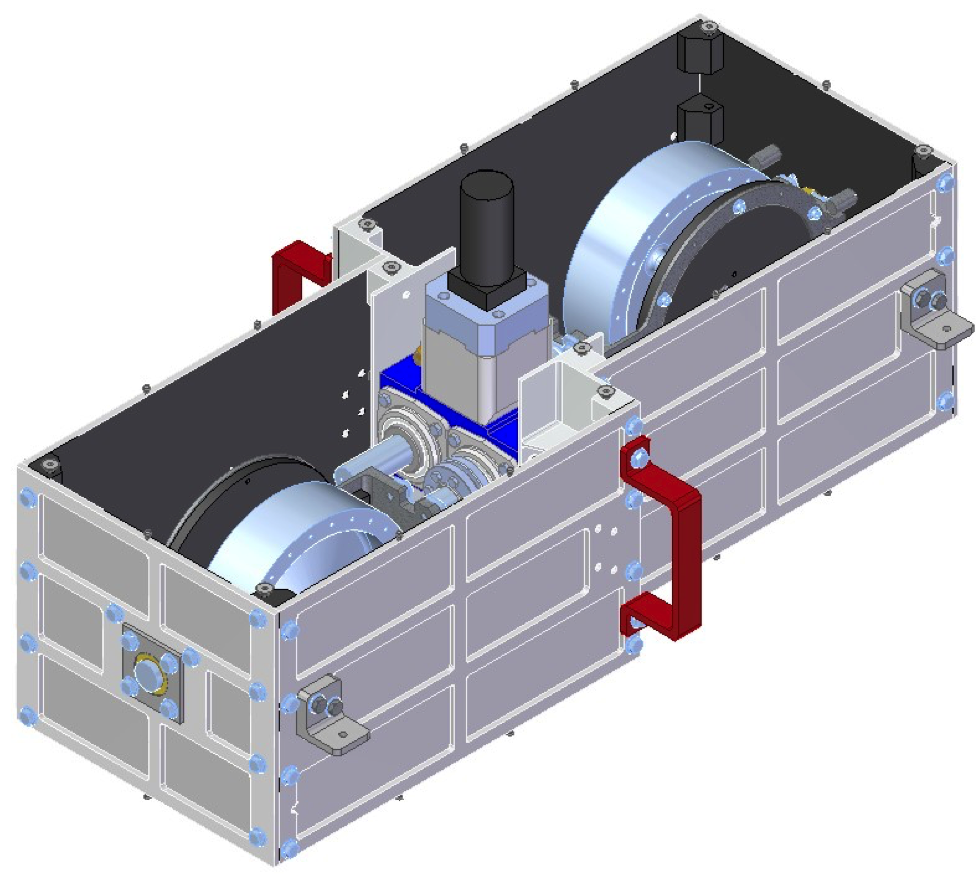
\includegraphics[width=\textwidth]{Figures/CCMG-case.png}
	\caption{}
	\label{fig:CCMGcase}
    \end{figure}


\subsection{Momentum dump mechanism}
\label{subsec:chap3momdumpmotor}
\subsection{Elevation control (Rotators)}
\subsection{Delay lines}
\subsection{Tip/tilt}
\subsection{Fine guidance sensor}


\subsection{Actuator description and characterization}
\subsection{Sensor description and characterization}
\subsubsection{Gyroscopes}
Set up the conditions of the test (attached to a slab of metal, and set on the ground); mention that we introduced a random phase noise to prevent spikes in the signal, due to the internal close-loop control of the gyroscopes
\begin{itemize}
\item Show the noise of each gyro; short timescales, high freq; long timescale, low freq;
\item Show the Allan variance for each gyro using R
\item Compare the noise PSD to a gaussian
\end{itemize}
\subsubsection{Encoders}
\subsubsection{Capacitive sensors}
\subsubsection{}
\subsection{Control electronics}
Clocks and timings \\
Computers
\subsection{Software architecture}
